\documentclass[11pt,a4paper]{article}

\usepackage[utf8]{inputenc}
\usepackage[T1]{fontenc}
\usepackage{lmodern}
\usepackage{geometry}
\usepackage{graphicx}
\usepackage{booktabs}
\usepackage{amsmath}
\usepackage{amssymb}
\usepackage{hyperref}
\usepackage{xcolor}
\usepackage{enumitem}
\usepackage{caption}
\usepackage{subcaption}

\geometry{margin=1in}
\hypersetup{
    colorlinks=true,
    linkcolor=blue,
    citecolor=blue,
    urlcolor=blue
}

\title{Representation Bias, Fast Simulation, and Efficient Evaluation for KTC2023 Electrical Impedance Tomography Reconstruction}
\author{Anonymous Authors}
\date{}

\begin{document}
\maketitle

\begin{abstract}
The Kuopio Tomography Challenge 2023 (KTC2023) provides a realistic benchmark for electrical impedance tomography (EIT) reconstruction from 32-electrode boundary measurements. In this work, we summarize a complete repository-scale study of KTC2023 reconstruction, covering simulation acceleration, efficient evaluation, and a systematic comparison of several representation families. We first optimize the synthetic data generation pipeline. By exploiting the reduced rank of the excitation matrix, we obtain an exact reduced-right-hand-side solve with a measured 5.11$\times$ speedup over the original direct forward solve. Combined with sparse assembly refinements, projection-matrix precomputation, and solver improvements, the complete per-sample generation pipeline is reduced from approximately 23.2 s to 117 ms. We also accelerate the official challenge score with a Torch/CUDA implementation whose single-sample runtime is reduced from approximately 92 s to 2.32 ms with negligible numerical deviation. On the reconstruction side, we compare FCUNet, post-processing, conditional diffusion, sparse autoencoding, vector-quantized autoencoding, and fixed-basis DCT prediction. The strongest reproduced overall benchmark score is obtained by the post-processing baseline at 16.028, while the proposed DCT ensemble reaches 14.055 and slightly surpasses the FCUNet baseline at 14.049 among direct measurement-driven methods. The study shows that fixed low-frequency representations offer a favorable balance between image regularity, predictability from measurements, and computational efficiency, whereas high-entropy latent spaces remain difficult to infer reliably from EIT data.
\end{abstract}

\noindent\textbf{Keywords:} electrical impedance tomography, KTC2023, low-frequency prior, DCT, simulation acceleration

\section{Introduction}
Electrical impedance tomography reconstructs an internal conductivity distribution from boundary current-voltage measurements and is well known to be nonlinear, ill-posed, and highly sensitive to modeling error \cite{cheney1999eit}. The KTC2023 benchmark \cite{rasanen2023kuopio} is a particularly useful evaluation setting because it combines real water-tank measurements, increasing difficulty levels, and a structured official metric based on class-wise similarity.

The central question in this study is not only which network gives the highest score, but also which \emph{representation bias} is best matched to the information content of EIT measurements. We therefore examined three classes of design choices: direct image-space prediction, learned latent-space inversion, and fixed analytical low-frequency decoding. At the same time, we optimized the engineering foundation needed for such a study, namely large-scale synthetic data generation and evaluation throughput.

The resulting picture is clear. First, engineering optimization matters: exact reduced-right-hand-side forward solving and end-to-end synthetic pipeline acceleration drastically increase iteration speed and make broader data-centric experiments feasible. Second, not all reconstruction representations are equally compatible with EIT. Pixel-wise discrete prediction and high-entropy latent dictionaries can regularize image manifolds, but they remain difficult to infer from measurements. Third, a fixed DCT basis offers a robust middle ground and produces the best direct measurement-driven benchmark result in this repository.

The main contributions of this KTC2023-focused paper are:
\begin{enumerate}[leftmargin=1.5em]
    \item an exact reduced-rank forward-solving strategy for KTC2023 simulation that yields a measured 5.11$\times$ speedup;
    \item an optimized end-to-end synthetic generation pipeline whose per-sample runtime is reduced from approximately 23.2 s to 117 ms;
    \item a Torch/CUDA challenge scorer with roughly four orders of magnitude faster single-sample runtime than the official implementation;
    \item a unified empirical comparison of FCUNet, post-processing, diffusion, sparse autoencoding, vector-quantized autoencoding, and fixed-basis DCT prediction;
    \item a direct demonstration that low-frequency analytical decoding is easier to infer from EIT measurements than high-entropy learned latent spaces.
\end{enumerate}

\section{Related Work}
\subsection{EIT Reconstruction}
Classical EIT inversion methods rely on regularized optimization and physics-based priors \cite{cheney1999eit,adler2006eidors}. Deep learning methods aim to amortize the inverse mapping, typically through direct image prediction, post-processing of classical reconstructions, or generative refinement.

\subsection{Neural KTC2023 Baselines}
The KTC2023 ecosystem already includes several strong paradigms: FCUNet-style direct reconstruction based on an image-space decoder \cite{chen2020deep}, post-processing of Tikhonov-type reconstructions \cite{martin2017post}, and diffusion-based conditional reconstruction. These methods provide strong baselines, but they also highlight the importance of representation choice.

\subsection{Low-Frequency and Latent Representations}
Low-frequency analytical bases such as the DCT \cite{ahmed1974dct} can impose global smoothness and structural coupling without introducing an additional learned decoder. In contrast, latent autoencoders and vector-quantized models \cite{oord2017vqvae} constrain the image manifold through a learned latent space. The key question is whether these latent spaces are also easy to recover from boundary measurements.

\section{Engineering Foundation}
\subsection{Exact Reduced-Rank Forward Solving}
The KTC2023 reference excitation matrix has 76 nominal right-hand sides, but its numerical rank is only 15. We used this fact to solve the complete electrode model in a reduced basis and reconstruct the full measurement matrix exactly afterward. The best benchmarked configuration is:
\begin{itemize}[leftmargin=1.5em]
    \item original direct solve: 298.57 ms/sample,
    \item exact reduced-right-hand-side solve: 58.47 ms/sample,
    \item measured speedup: 5.11$\times$.
\end{itemize}

These numbers come from:
\begin{itemize}[leftmargin=1.5em]
    \item \texttt{../../results/forward\_batched\_pcg\_torch\_cached\_svd\_l1\_n5\_1/summary.json}
\end{itemize}

\subsection{End-to-End Synthetic Data Generation}
The reduced-rank forward solve is only one part of the full synthetic data generation pipeline. In the repository, each sample also includes linearized reconstruction, interpolation, and file-writing related work. We therefore further optimized the complete generation chain through sparse-matrix assembly improvements, projection-matrix precomputation, and solver replacement. The cumulative result is:
\begin{itemize}[leftmargin=1.5em]
    \item original total pipeline: 23210 ms/sample,
    \item optimized total pipeline: 117 ms/sample,
    \item cumulative speedup: approximately 198$\times$.
\end{itemize}

These numbers are summarized in:
\begin{itemize}[leftmargin=1.5em]
    \item \texttt{../../GUIDE/data\_generation\_optimization.md}
\end{itemize}

This end-to-end reduction is important because it changes the practical scale of experimentation. Without it, large simulation-driven ablation studies on data size, representation choice, and model families would be prohibitively slow.

\subsection{Fast KTC Scoring}
The official KTC score is computationally expensive because it repeatedly evaluates class-wise SSIM on full-resolution images. We implemented fast SciPy and Torch/CUDA versions and benchmarked them on a real challenge sample. The best Torch/CUDA cached implementation achieves:
\begin{itemize}[leftmargin=1.5em]
    \item official: 92015 ms/sample,
    \item fast SciPy: 127.28 ms/sample,
    \item fast Torch/CUDA cached: 2.32 ms/sample,
    \item absolute score difference versus official: $5.41\times10^{-7}$.
\end{itemize}

The benchmark source is:
\begin{itemize}[leftmargin=1.5em]
    \item \texttt{../../results/scoring\_benchmark\_2/summary.json}
\end{itemize}

\section{Methods}
\subsection{FCUNet}
FCUNet maps the flattened 2356-dimensional measurement vector to a coarse spatial map and refines it with a U-Net decoder \cite{ronneberger2015unet}. It is the strongest direct benchmark baseline in the current repository.

\subsection{Post-Processing and Diffusion Baselines}
The post-processing baseline predicts the final segmentation from physics-based initial reconstructions rather than directly from measurements. The conditional diffusion baseline similarly operates on reconstruction-space conditioning. These methods are important comparators because they exploit more structure than a purely direct measurement-to-image mapping.

\subsection{Latent Autoencoding Routes}
We examined two latent routes:
\begin{itemize}[leftmargin=1.5em]
    \item a sparse autoencoder (SAE) that learns a compact continuous latent;
    \item a structured 1D vector-quantized autoencoder that uses a discrete codebook and canonical pose alignment.
\end{itemize}
In both cases the decoder can reconstruct reasonable images from true latent variables, but the inverse mapping from measurements to latent codes remains unreliable.

\subsection{Fixed-Basis DCT Predictor}
The DCT predictor directly regresses a small block of low-frequency DCT coefficients from the measurement vector and reconstructs class logits with a fixed inverse DCT. This avoids learning a separate high-entropy decoder and imposes a global low-frequency prior explicitly. We also evaluate a lightweight two-model ensemble that averages logits from two independently trained DCT predictors.

\section{Experimental Setup}
\subsection{Dataset and Metric}
We use the KTC2023 training and evaluation materials \cite{rasanen2023kuopio}. The benchmark provides 32-electrode measurements, 76 injection patterns, and three-class target segmentations. Final evaluation uses the official class-wise SSIM-based challenge score.

\subsection{Compared Methods}
The reproduced methods considered in this paper are:
\begin{itemize}[leftmargin=1.5em]
    \item FCUNet,
    \item Post-processing,
    \item Conditional diffusion,
    \item DPCAUNet,
    \item HC-DPCA-UNet,
    \item SAE-based predictor,
    \item DCT predictor,
    \item DCT predictor ensemble.
\end{itemize}

\section{Results}
\subsection{Main Benchmark Comparison}
Table~\ref{tab:ktc-main} summarizes the main reproduced benchmark results.

\begin{table}[htbp]
    \centering
    \caption{KTC2023 official benchmark comparison.}
    \label{tab:ktc-main}
    \begin{tabular}{lc}
        \toprule
        Method & Total score \\
        \midrule
        Post-processing & \textbf{16.028} \\
        DCT predictor ensemble & 14.055 \\
        FCUNet & 14.049 \\
        DCT predictor & 13.980 \\
        SAE predictor & 5.230 \\
        HC-DPCA-UNet & 4.259 \\
        DPCAUNet & 2.804 \\
        Conditional diffusion & 7.976 \\
        \bottomrule
    \end{tabular}
\end{table}

The table leads to three immediate observations. First, post-processing remains the strongest reproduced overall route in this repository. Second, the DCT ensemble is slightly stronger than FCUNet and is therefore the best current direct measurement-driven method in our codebase. Third, high-entropy latent and pixel-wise discrete routes lag far behind despite often producing visually smoother intermediate reconstructions.

\subsection{Representation Comparison}
The KTC study repeatedly showed that decoder regularity alone is not enough. SAE and VQ-style models can reconstruct benchmark phantoms from true latent variables, but the learned measurement-to-latent inversion remains weak. In contrast, the fixed DCT basis reduces the prediction target to a small, globally coupled, low-frequency coefficient set that is substantially easier to infer from measurements.

Qualitative comparison across methods is illustrated in Figure~\ref{fig:ktc-qualitative}.

\begin{figure}[htbp]
    \centering
    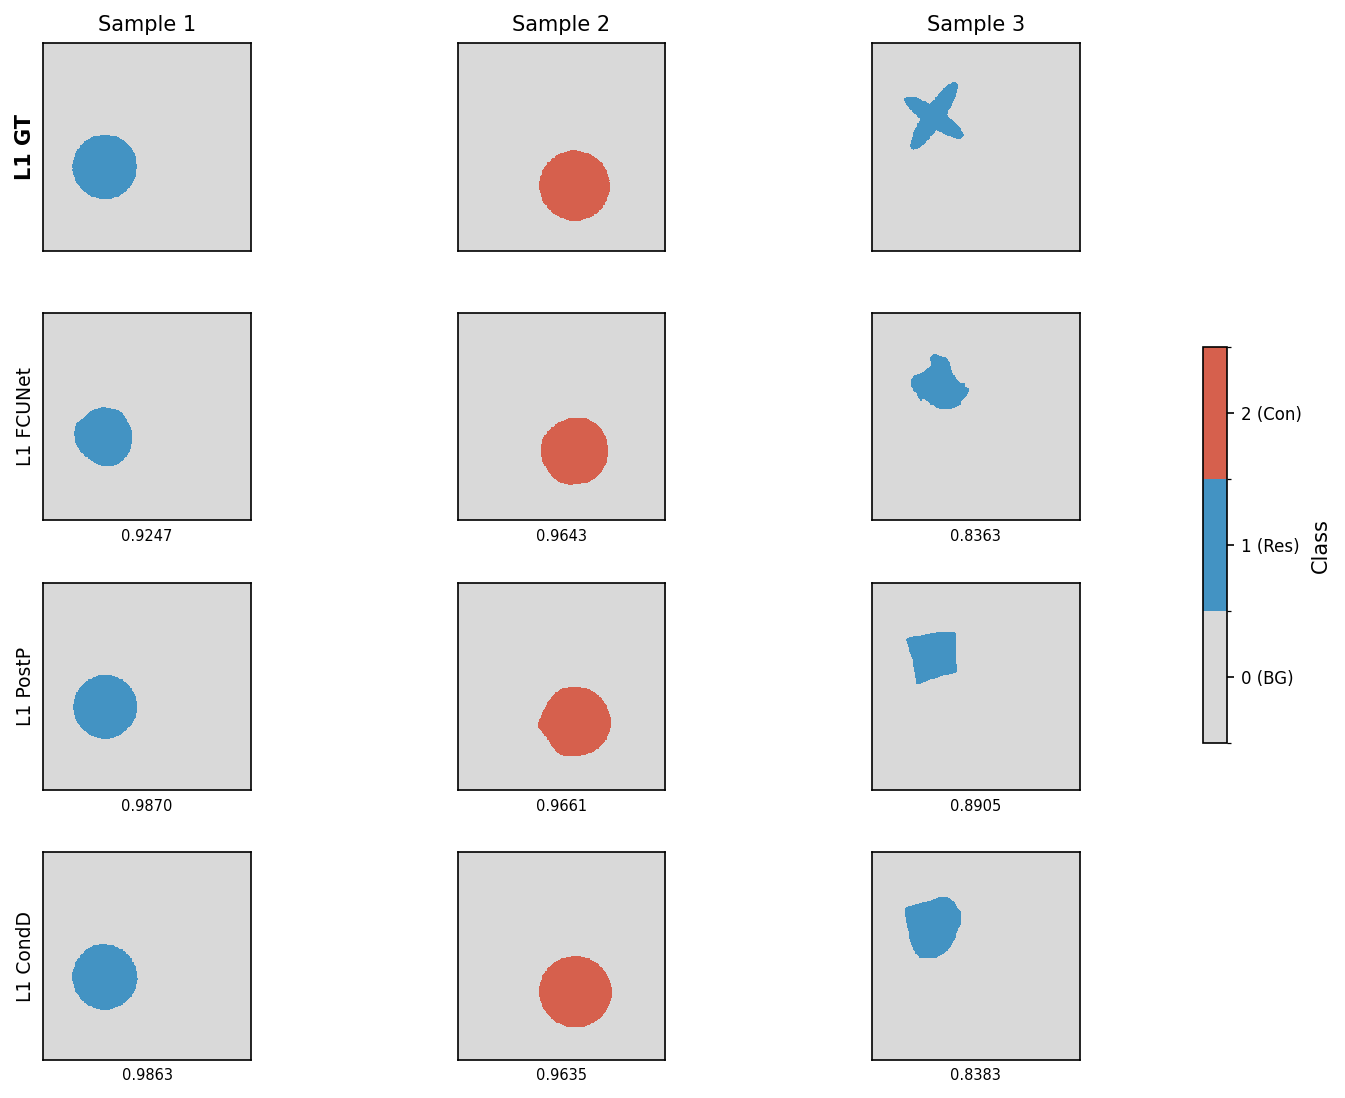
\includegraphics[width=0.92\linewidth]{../../results/cross_method_comparison.png}
    \caption{Representative KTC2023 cross-method comparison using repository-generated benchmark visualizations.}
    \label{fig:ktc-qualitative}
\end{figure}

\subsection{Data Scaling and Benchmark Efficiency}
The repository also contains a training-data scaling study for FCUNet. As the synthetic training set grows from 100 to 6400 samples, the synthetic test score improves from 0.735 to 0.921. This confirms that data availability strongly affects learned EIT reconstruction, although synthetic-to-real transfer on the official challenge remains imperfect.

\begin{figure}[htbp]
    \centering
    \begin{subfigure}{0.48\linewidth}
        \centering
        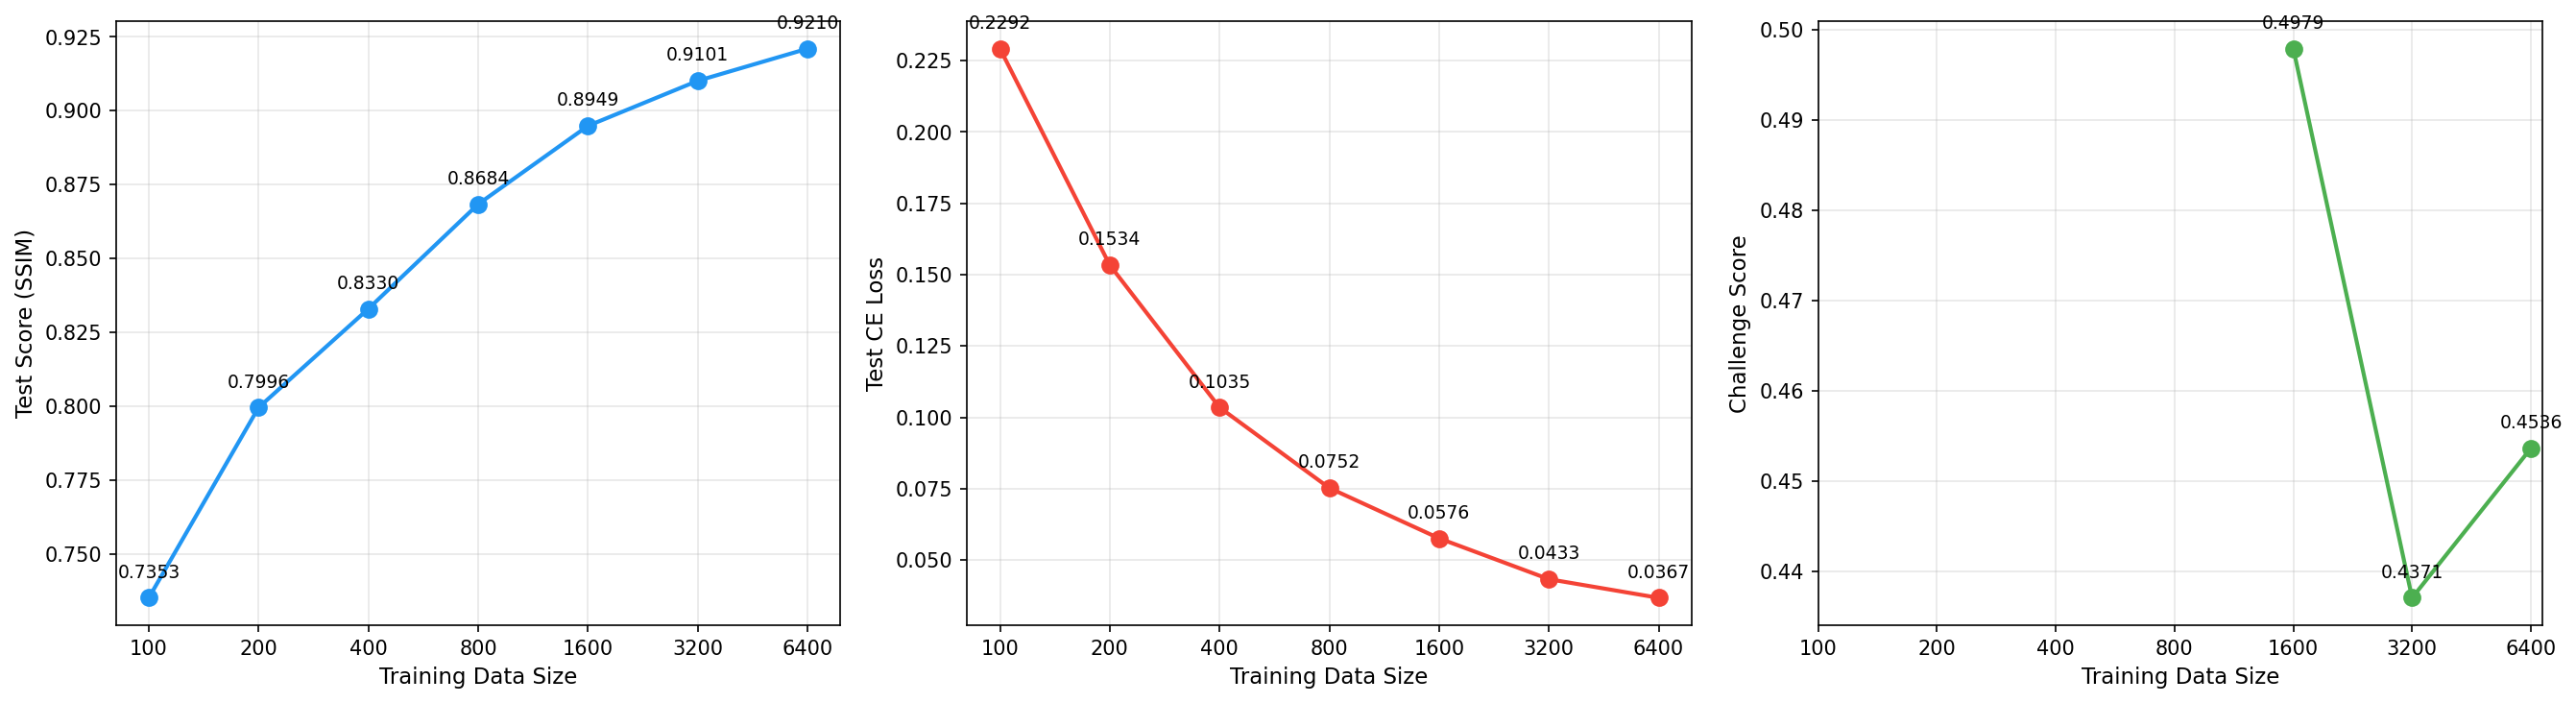
\includegraphics[width=\linewidth]{../../results/data_scaling_comparison.png}
    \end{subfigure}
    \hfill
    \begin{subfigure}{0.48\linewidth}
        \centering
        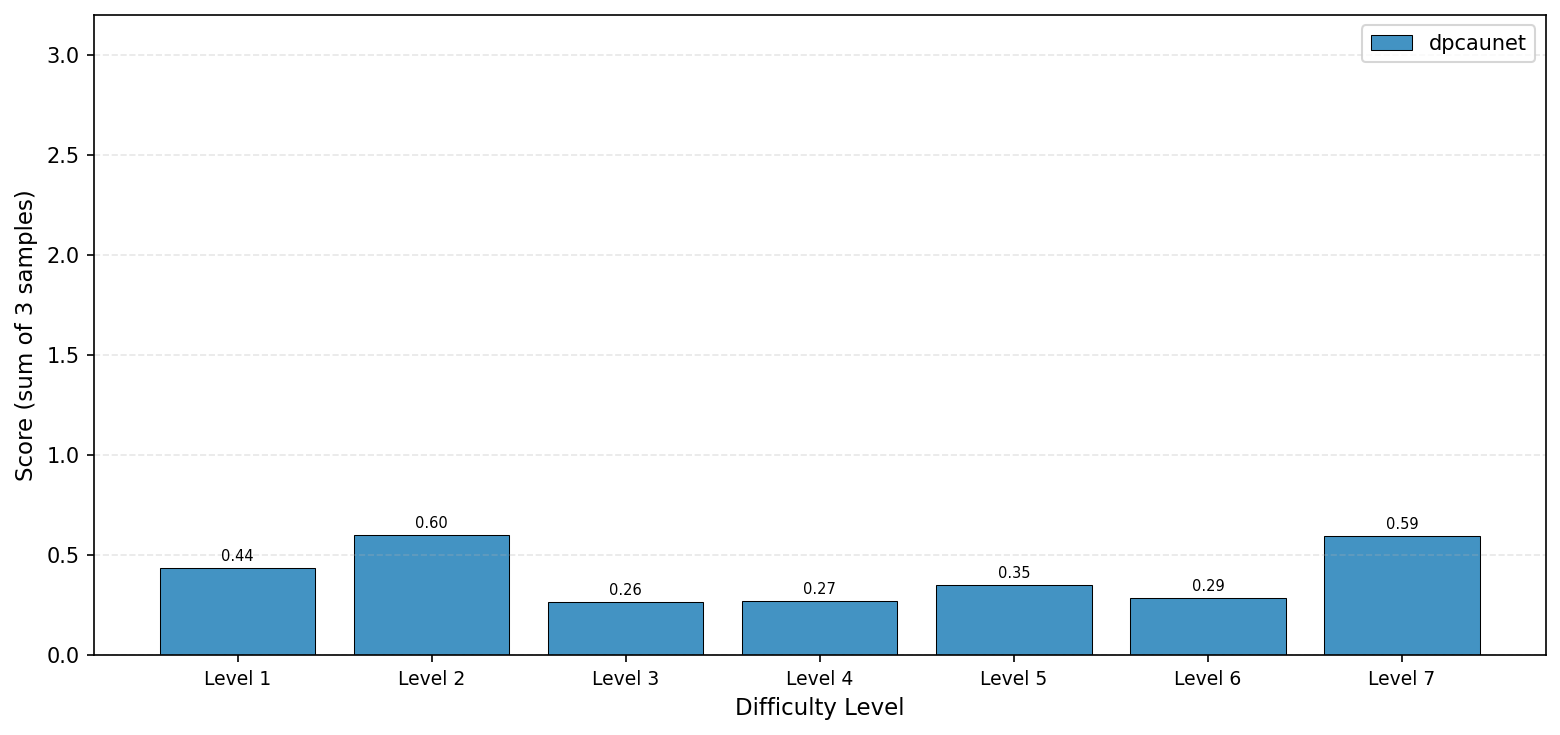
\includegraphics[width=\linewidth]{../../results/scores_bar_chart.png}
    \end{subfigure}
    \caption{Repository-generated KTC2023 summary figures. Left: data-scaling trend for FCUNet. Right: score comparison across reproduced methods.}
    \label{fig:ktc-scaling}
\end{figure}

\section{Discussion}
The KTC2023 study provides a useful separation between image regularity and inverse-map predictability. Pixel-wise discrete models and latent autoencoders can constrain the image manifold, but they do not automatically make the inverse map easier. The DCT route succeeds because it directly encodes the kind of global low-frequency structure that is both consistent with the target images and statistically recoverable from boundary measurements.

At the same time, the benchmark also shows that direct measurement-driven reconstruction is not always the strongest overall strategy. Post-processing of physics-based reconstructions remains highly competitive and currently gives the best reproduced total score in this repository. Therefore, the strongest conclusion is not that DCT universally dominates, but that DCT is the best current \emph{direct} reconstruction route and offers a compelling tradeoff between simplicity, regularity, and accuracy.

\section{Conclusion}
This paper summarized a complete KTC2023-focused research cycle on the current codebase. The main conclusions are:
\begin{itemize}[leftmargin=1.5em]
    \item exact reduced-right-hand-side forward solving yields a measured 5.11$\times$ simulation speedup without changing the underlying physics;
    \item the complete synthetic generation pipeline is reduced from approximately 23.2 s to 117 ms per sample, making large-scale simulation studies practical;
    \item Torch/CUDA scoring reduces single-sample evaluation time from approximately 92 s to 2.32 ms with negligible score deviation;
    \item among reproduced direct measurement-driven methods, the DCT ensemble is currently strongest at 14.055, slightly surpassing FCUNet at 14.049;
    \item post-processing remains the strongest reproduced overall benchmark baseline at 16.028;
    \item fixed analytical low-frequency decoding is substantially easier to invert from measurements than high-entropy learned latent spaces.
\end{itemize}

These results make the KTC2023 benchmark side of the project mature enough to stand alone as a completed study. They also motivate the pulmonary extension: if low-frequency analytical priors are effective on structured phantom reconstruction, the next question is how far they transfer to anatomically constrained pulmonary EIT.

\bibliographystyle{plain}
\bibliography{references}

\end{document}
